% ------------------------------------------------------------------------------
% TYPO3 CMS 7.1 - What's New - Chapter "Introduction" (Serbian Version)
%
% @author	Michael Schams <schams.net>
% @license	Creative Commons BY-NC-SA 3.0
% @link		http://typo3.org/download/release-notes/whats-new/
% @language	Serbian
% ------------------------------------------------------------------------------
% LTXE-CHAPTER-UID:		947f71fe-f93742b1-4879d61a-4a9bbcd6
% LTXE-CHAPTER-NAME:	Introduction
% ------------------------------------------------------------------------------

\section{Uvod}
\begin{frame}[fragile]
	\frametitle{Uvod}

	\begin{center}\huge{Uvod}\end{center}
	\begin{center}\huge{\color{typo3darkgrey}\textbf{Cinjenice}}\end{center}

\end{frame}

% ------------------------------------------------------------------------------
% LTXE-SLIDE-START
% LTXE-SLIDE-UID:		43d80e7d-a67b9387-093f341d-f18d266b
% LTXE-SLIDE-ORIGIN:	a86a13ef-338d870a-beaf8e5a-65cd0eab English
% LTXE-SLIDE-TITLE:		TYPO3 CMS 7.1 - Die Fakten
% ------------------------------------------------------------------------------

\begin{frame}[fragile]
	\frametitle{Uvod}
	\framesubtitle{TYPO3 CMS 7.1 - Cinjenice}

	\begin{itemize}
		\item Datum objavljivanja: 24. februar 2015.
		\item Tip objavljivanja: "Brza objava" ("Sprint Release")
		\item Vizija: Prihvatiti, inovirati, dostaviti
		\item Glavni fokus: Ciscenje osnove sistema i optimizacija
	\end{itemize}

	\begin{figure}
		
\includegraphics[width=0.95\linewidth]{typo3-seven-zero-banner.png}
	\end{figure}

\end{frame}

% ------------------------------------------------------------------------------
% LTXE-SLIDE-START
% LTXE-SLIDE-UID:		4c8aa58a-f87885be-83771fb6-353729b8
% LTXE-SLIDE-ORIGIN:	37e4488f-040dd53e-fac4a3a3-c587b0d9 English
% LTXE-SLIDE-TITLE:		System Requirements
% ------------------------------------------------------------------------------

\begin{frame}[fragile]
	\frametitle{Uvod}
	\framesubtitle{Sistemski zahtevi}

	\begin{itemize}
		\item PHP*:\tabto{3cm}v5.5.0 - v5.6.x
		\item MySQL:\tabto{3cm}v5.5.x - v5.6.x (no strict mode)
		\item Prostor na disku:\tabto{3cm}min 200 MB
		\item PHP podesavanja:

			\begin{itemize}
				\item memory\_limit >= 128M
				\item max\_execution\_time >= 240s
				\item opcija \texttt{--disable-ipv6} se \underline{ne} sme korisiti
			\end{itemize}

		\item Administratorski interfejs zahteva IE >= 9 ili bilo koji drugi moderni pretrazivac

	\end{itemize}

	\vspace{0.5cm}
	*) Dodatno objasnjenje: \href{http://typo3.org/news/article/php-minimum-requirements-for-typo3-cms-7/}{PHP minimalni zahtevi za TYPO3 CMS 7}

\end{frame}

% ------------------------------------------------------------------------------
% LTXE-SLIDE-START
% LTXE-SLIDE-UID:		464b7a7b-5c43e58e-7f05b634-2d8aedaa
% LTXE-SLIDE-ORIGIN:	249e8dc9-e935b8a6-999d6e0b-c66c33b6 English
% LTXE-SLIDE-TITLE:		Development And Release Timeline
% ------------------------------------------------------------------------------

\begin{frame}[fragile]
	\frametitle{Uvod}
	\framesubtitle{Vreme razvoja i datumi objavljivanja}

	\begin{figure}
		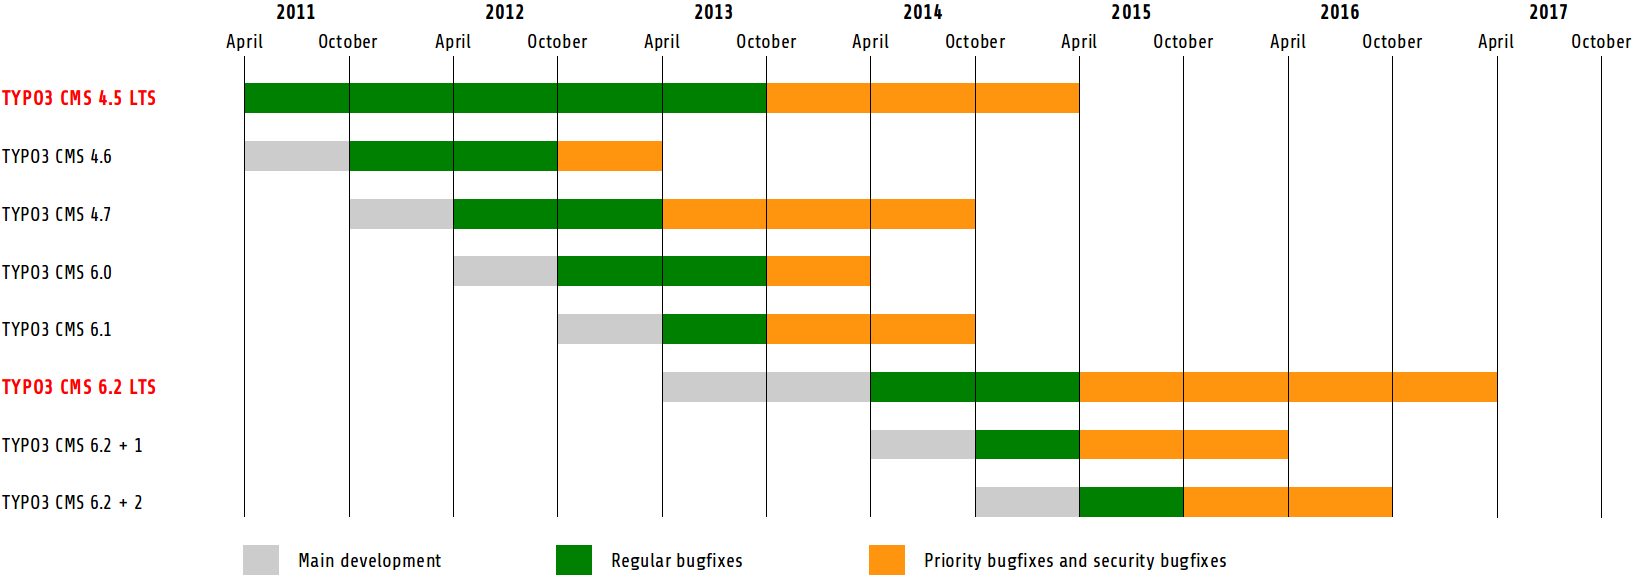
\includegraphics[width=0.90\linewidth]{Introduction/ReleaseAgenda.png}
	\end{figure}

\end{frame}

% ------------------------------------------------------------------------------
% LTXE-SLIDE-START
% LTXE-SLIDE-UID:		4c43d131-83c3391e-b412331b-9777031c
% LTXE-SLIDE-ORIGIN:	855168a2-d07a3cc8-65f8f9bd-827ef9e9 English
% LTXE-SLIDE-TITLE:		TYPO3 CMS Roadmap
% ------------------------------------------------------------------------------
% https://typo3.org/typo3-cms/roadmap/

\begin{frame}[fragile]
	\frametitle{Uvod}
	\framesubtitle{TYPO3 CMS plan}

	Predvidjeni datumi objavljivanja i njihov osnovni fokus:

	\begin{itemize}
		\item v7.0 \textrightarrow\tabto{1.3cm}02/Dec/2014\tabto{3.4cm}Remont administratorskog interfejsa prvi deo

		\item
			\begingroup
				\color{typo3orange}
					v7.1 \textrightarrow\tabto{1.3cm}24/Feb/2015\tabto{3.4cm}Ciscenje osnove sistema i optimizacija
			\endgroup

		\item v7.2 \textrightarrow\tabto{1.3cm}10/Mar/2015\tabto{3.4cm}Korisnicki interfejs
		\item v7.3 \textrightarrow\tabto{1.3cm}21/Apr/2015\tabto{3.4cm}Composer Ecosystem
		\item v7.4 \textrightarrow\tabto{1.3cm}09/Jun/2015\tabto{3.4cm}Remont administratorskog interfejsa drugi deo
		\item v7.5 \textrightarrow\tabto{1.3cm}28/Jul/2015\tabto{3.4cm}\textit{(bice odredjeno...)}
		\item v7.6 \textrightarrow\tabto{1.3cm}13/Oct/2015\tabto{3.4cm}Priprema LTS verzije
		\item v7.7 \textrightarrow\tabto{1.3cm}xx/xxx/2015\tabto{3.4cm}\textbf{TYPO3 CMS 7 LTS} (Verzija sa dugorocnom podrskom)
	\end{itemize}

	\smaller
		\url{https://typo3.org/typo3-cms/roadmap/}\newline
		\url{http://typo3.org/news/article/embrace-and-innovate-typo3-cms-7/}
	\normalsize

\end{frame}

% ------------------------------------------------------------------------------
% LTXE-SLIDE-START
% LTXE-SLIDE-UID:		acdf1a6b-c0d4c9fd-789a2234-3778ee55
% LTXE-SLIDE-ORIGIN:	0a54fbe0-06a2837d-605a5eed-6aa40506 English
% LTXE-SLIDE-TITLE:		Installation
% LTXE-SLIDE-REFERENCE:	https://forge.typo3.org/issues/62578
% ------------------------------------------------------------------------------

\begin{frame}[fragile]
	\frametitle{Uvod}
	\framesubtitle{Instalacija}

	\begin{itemize}
		\item Zvanicna procedura za instalaciju na Linux/Mac OS X\newline
			(DocumentRoot na primer \texttt{/var/www/site/htdocs}):
		\begin{lstlisting}
			$ cd /var/www/site
			$ wget --content-disposition get.typo3.org/7.1
			$ tar xzf typo3_src-7.1.0.tar.gz
			$ cd htdocs
			$ ln -s ../typo3_src-7.1.0 typo3_src
			$ ln -s typo3_src/index.php
			$ ln -s typo3_src/typo3
			$ touch FIRST_INSTALL
		\end{lstlisting}

		\item Simbolicki linkovi (Symbolic links) na Microsoft Windows:

			\begin{itemize}
				\item Koristiti \texttt{junction} za Windows XP/2000
				\item Koristiti  \texttt{mlink} za Windows Vista i Windows 7
			\end{itemize}

	\end{itemize}
\end{frame}

% ------------------------------------------------------------------------------
% LTXE-SLIDE-START
% LTXE-SLIDE-UID:		85c587aa-c70fe37a-44837e7f-c5e04603
% LTXE-SLIDE-ORIGIN:	914dda49-a07eaf35-b9d24c58-6890a673 English
% LTXE-SLIDE-TITLE:		Upgrade to TYPO3 CMS 7
% LTXE-SLIDE-REFERENCE:	https://forge.typo3.org/issues/62578
% ------------------------------------------------------------------------------

\begin{frame}[fragile]
	\frametitle{Uvod}
	\framesubtitle{Nadogradnja na TYPO3 CMS 7.x}

	\begin{itemize}
		\item Nadogradnja je moguca samo sa TYPO3 CMS 6.2 LTS
		\item TYPO3 CMS < 6.2 bi prvo trebalo nadograditi na TYPO3 CMS 6.2 LTS
	\end{itemize}

	\begin{itemize}

		\item Upsutstvo za nadogradnju:\newline
			\smaller\url{http://wiki.typo3.org/Upgrade#Upgrading_to_7.1}\normalsize
		\item Zvanicni TYPO3 vodic "TYPO3 Installation and Upgrading":
			\smaller\url{http://docs.typo3.org/typo3cms/InstallationGuide}\normalsize
		\item Opsti pristup:
			\begin{itemize}
				\item Proveriti minimalne sistemske zahte \small(PHP, MySQL, etc.)
				\item Proveriti \textbf{deprecation\_*.log} u staroj TYPO3 instanci
				\item Nadograditi sva prosirenja na najnoviju verziju
				\item Postaviti nove fajlove i pokrenuti Install Tool \textrightarrow Upgrade Wizard
				\item Proveriti startup modul za administratore (opciono)
			\end{itemize}
	\end{itemize}

\end{frame}

% ------------------------------------------------------------------------------
